
\documentclass[a4]{beamer}
\usepackage{amssymb}
\usepackage{graphicx}
\usepackage{subfigure}
\usepackage{newlfont}
\usepackage{amsmath,amsthm,amsfonts}
%\usepackage{beamerthemesplit}
\usepackage{pgf,pgfarrows,pgfnodes,pgfautomata,pgfheaps,pgfshade}
\usepackage{mathptmx} % Font Family
\usepackage{helvet} % Font Family
\usepackage{color}
\mode<presentation> {
\usetheme{Default} % was Frankfurt
\useinnertheme{rounded}
\useoutertheme{infolines}
\usefonttheme{serif}
%\usecolortheme{wolverine}
% \usecolortheme{rose}
\usefonttheme{structurebold}
}
\setbeamercovered{dynamic}
\title[MA4413]{Statistics for Computing \\ {\normalsize MA4413 Lecture 10B}}
\author[Kevin O'Brien]{Kevin O'Brien \\ {\scriptsize Kevin.obrien@ul.ie}}
\date{Autumn Semester 2013}
\institute[Maths \& Stats]{Dept. of Mathematics \& Statistics, \\ University \textit{of} Limerick}

\renewcommand{\arraystretch}{1.5}
%----------------------------------------------------------------------------------------------------------%
\begin{document}


\titlepage



\noindent \textbf{Inference Procedures with \texttt{R}}



\noindent \textbf{The paired t-test with \texttt{R}}
\vspace{-1cm}
\begin{itemize}
\item Previously we have seen the paired $t-$test. It is used to determine whether or
not there is a significant difference between paired measurements. \item Equivalently whether or not
the case-wise differences are zero.
\item The mean and standard deviation of the case-wise differences are used to determine the test statistic.
\item Under the null hypothesis, the expected value of the case-wise differences is zero (i.e $H_0 : \mu_d = 0$).
%\item The test statistic is computed as
%\[ TS = \frac{\bar{d} - \mu_d}{\frac{s_d}{\sqrt{n}}} \]
\end{itemize}




%------------------------------------------%
[fragile]
\noindent \textbf{The paired t-test with \texttt{R}}
%Alternative Approach : using p-values.
\begin{itemize}
\item Conclusions about all inference procedures can be made based on the $p-$values.
\item The p-values can be determined from computer code. (We will use a software called \texttt{R}. Other types of software inlcude \texttt{SAS} and \texttt{SPSS}.)
%\item The null and alternative are as before.
\item The computer software automatically generates the appropriate test statistic, and hence the corresponding $p-$value.
\item The user then interprets the $p-$values. If $p-$value is small, reject the null hypothesis. If the p-value is large, the appropriate conclusion is a failure to reject $H_0$.
\item The threshold for being considered small is less than $\alpha/k$, usually 0.0250. \\ (This is actually a very arbitrary choice of threshold, suitable for some subject areas, not for others.)
\end{itemize}

%------------------------------------------%
[fragile]
\noindent \textbf{The paired t-test with \texttt{R}}

\begin{itemize}
\item In the following procedure (next slide), there are two sets of values: the \texttt{Before} values and the \texttt{After} values.
\item The \texttt{R} command is \texttt{t.test()}, with the additional specification ``\texttt{paired=}".
\item The alternative hypothesis is specified in the output. ( Another way of expressing it: True mean of case-wise differences is not zero)
\item Also included in the output is a 95\% confidence interval for the sample mean of case-wise differences.
\end{itemize}

%------------------------------------------%
[fragile]
\noindent \textbf{The paired t-test with \texttt{R}}
Implementing the paired t-test using \texttt{R} for the example previously discussed.
\begin{verbatim}
> t.test(Before,After,paired=TRUE)

        Paired t-test

data:  Before and After
t = 3.8881, df = 13, p-value = 0.001868
alternative hypothesis: true difference in means is not 0
95 percent confidence interval:
  3.650075 12.778496
sample estimates:
mean of the differences
               8.214286

\end{verbatim}


%-------------------------------------------------%
[fragile]
\noindent \textbf{The paired t-test with \texttt{R}}
\begin{itemize}
\item The p-value ($0.001868$) is less than the threshold is less than the threshold $0.0250$.
\item We reject the null hypothesis (mean of case-wise differences being zero, i.e. expect no difference between ``before" and ``after").
\item We conclude that there is a likely to be a difference between `before' and `after' measurements.
\item That is to say, we can expected a difference between two paired measurements.
\end{itemize}

%-------------------------------------------------%
[fragile]
\noindent \textbf{The paired t-test with \texttt{R}}
\begin{itemize}
\item We could also consider the confidence interval. We are $95\%$ confident that the expected value of the case-wise difference is at least 3.65.
\item Here the null value (i.e. 0) is not within the range of the confidence limits.
\item Therefore we reject the null hypothesis.
\end{itemize}
\begin{verbatim}
> t.test(Before,After,paired=TRUE)
...
...
95 percent confidence interval:
  3.650075 12.778496
...
\end{verbatim}







%-------------------------------------------------%
[fragile]
\noindent \textbf{Graphical Procedures for assessing Normality}

\begin{itemize}
\item The normal probability (Q-Q) plot is a very useful tool for determining whether or not a data set is normally distributed.
\item Interpretation is simple. If the points follow the trendline (provided by the second line of \texttt{R} code \texttt{qqline}), then the data set can be assumed to be normally distributed.
\item One should expect minor deviations. Numerous major deviations would lead the analyst to conclude that the data set is not normally distributed.
\item The Q-Q plot is best used in conjunction with a formal procedure such as the Shapiro-Wilk test.
\end{itemize}

\begin{verbatim}
>qqnorm(CWdiff)
>qqline(CWdiff)
\end{verbatim}



%-------------------------------------------------%


\noindent \textbf{Graphical Procedures for Assessing Normality}

\begin{center}
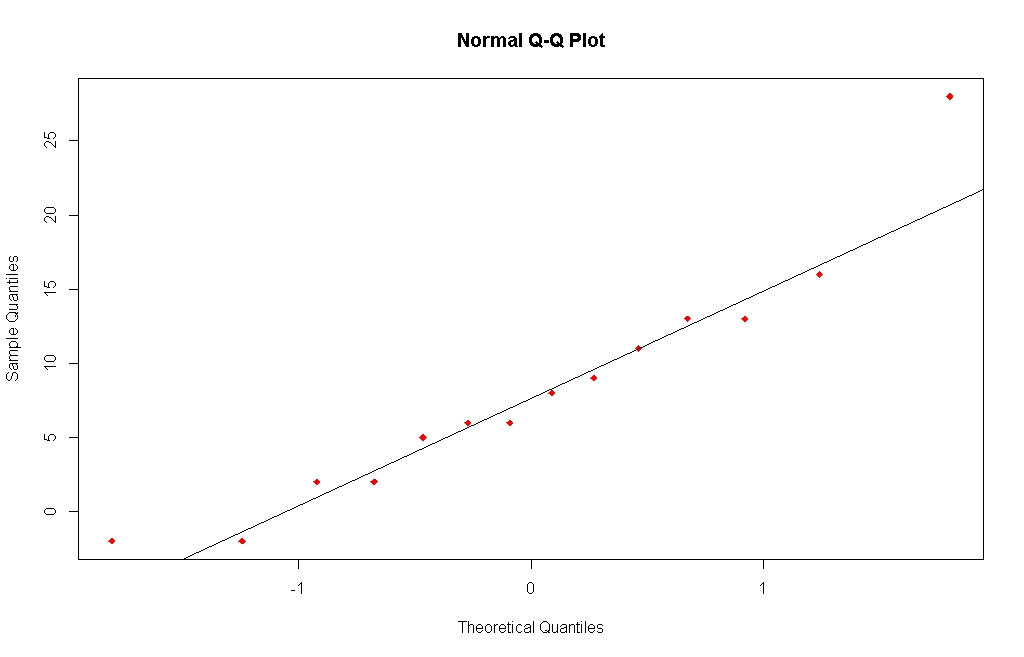
\includegraphics[scale=0.32]{10AQQplot}
\end{center}

%----------------------------------------------------------%
[fragile]
\noindent \textbf{Grubbs Test for Determining an Outlier}

\begin{itemize}
\item The Grubbs test is used to determine if there is exactly one outlier in a complete data set.
\item (This is actually the most common of several variants of the Grubbs' test).
\item Importantly, the test requires that the data is normally distributed to be a valid approach.
\item There is no agreed formal definition for an outlier. The definition of outlier used for this procedure is a value that unusually distance from the rest of the values.
\item (For the sake of clarity , we shall call this type of outlier a \textbf{Grubbs Outlier}). 
\end{itemize}


%-------------------------------------------------%
[fragile]
\noindent \textbf{Grubbs Test for Determining an Outlier}
Consider the following data set: is the lowest value (4.01) an outlier?
\begin{verbatim}
      6.98 8.49 7.97 6.64
      8.80 8.48 5.94 6.94
      6.89 7.47 7.32 4.01
\end{verbatim}

Under the null hypothesis, there is no outlier present in the data set. 
We reject this hypothesis if the $p-$value is sufficiently small.


%-------------------------------------------------%
[fragile]
\noindent \textbf{Grubbs Test for Determining an Outlier}
\vspace{-1cm}
\begin{verbatim}
> grubbs.test(x, two.sided=T)
Grubbs test for one outlier
data: x
G = 2.4093, U = 0.4243, p-value = 0.05069
alternative hypothesis: lowest value 4.01 is an outlier
\end{verbatim}
We conclude that while small by comparison to the other values, the lowest value 4.01 is not an outlier.


\end{document}


%-------------------------------------------------%
%-------------------------------------------------%
[fragile]
\noindent \textbf{Single Sample Proportion Test (a)}

\begin{itemize}
\item In this procedure, we determine whether or not we are are justified in assuming that the population proportion takes a certain value.
\item For example, suppose we believed that the population proportion of students with iphones or androids was $80\%$.
\item We would write the null and alternative accordingly.
\[H_0 : \pi = 80\% \]
\[H_1 : \pi \neq 80\% \]
\item The  appropriate \texttt{R} command is \texttt{prop.test(x,n,p)}
\item $x$ is the number of successes, $n$ is the sample size and $p$ is the population proportion assumed under the null hypothesis.
\item Suppose we survey 65 students, with 50 replying that they had an iphone or android.
\end{itemize}


%-------------------------------------------------%

[fragile]
\noindent \textbf{Single Sample Proportion Test (b)}

\begin{verbatim}
> prop.test(50,65,0.80)

        1-sample proportions test

data:  50 out of 65, null probability 0.8
X-squared = 0.2163, df = 1, p-value = 0.6418
alternative hypothesis: true p is not equal to 0.8
95 percent confidence interval:
 0.6452269 0.8610191
sample estimates:
        p
0.7692308
\end{verbatim}



[fragile]
\noindent \textbf{Single Sample Proportion Test (c)}

\begin{itemize}
\item The p-value is above the threshold. Therefore we fail to reject the null hypothesis that the population proportion ($\pi$) is $80\%$.

\item The observed proportion is a very straightforward calculation:

\[ \hat{p} = \frac{50}{65} = 0.76923= 76.92\%\]
\item Nonetheless, you would be required to show how it was calculated.
\end{itemize}



%-------------------------------------------------%
[fragile]
\noindent \textbf{Test of Equality for Two Sample Proportions (a)}
The null hypothesis is that two populations have the same proportions for a particular characteristic.
\[H_0 : \pi_1 = \pi_2 \]
\[H_1 : \pi_1 \neq \pi_2 \]
\begin{itemize}
\item The command is \texttt{prop.test(c(x1,x2),c(n1,n2))}
\item $x1$ and $x2$ are the number of successes from both samples.
\item $n2$ and $n2$ are the sample sizes for both groups.
\item The difference in population proportions assumed under the null hypothesis is zero.
\item (It is possible to specify a different null value, but we will not consider this in this module.)
\end{itemize}


%-------------------------------------------------%

\noindent \textbf{Test of Equality for Two Sample Proportions (b)}
\begin{itemize}
\item Consider a study where the proportion of Irish students who owned mobile devices, such as iphones and androids was compared to the corresponding proportion of French student.
\item As before, $65$ Irish students were interviewed, with $50$ replying that they owned mobile devices.
\item $90$ french students were interview, with 60 responding that they owned mobile devices.
\item The test of equality of proportions is implemented on the next slide.
\end{itemize}


%-------------------------------------------------%


[fragile]
\noindent \textbf{Test of Equality for Two Sample Proportions (c)}
Based on the p-value, we fail to reject the null hypothesis. There is not enough evidence to assume a difference in proportions. Also the expected difference assumed under the null hypothesis, i.e. 0, is contained in the confidence interval.
\begin{verbatim}
> prop.test(c(50,60),c(65,90))

        2-sample test for equality of proportions

data:  c(50, 60) out of c(65, 90)
X-squared = 1.4613, df = 1, p-value = 0.2267
alternative hypothesis: two.sided
95 percent confidence interval:
 -0.05202058  0.25714878
sample estimates:
   prop 1    prop 2
0.7692308 0.6666667
\end{verbatim}

[fragile]
\noindent \textbf{Test of Equality for Two Sample Proportions (d)}
\begin{itemize}
\item You would be required to compute the differences in observed proportions.
\item Additionally you will given the \texttt{R} code for one sample procedures. This may or may not be relevant for answering the question.
\end{itemize}
\begin{verbatim}
> prop.test(60,90,0.80)
...
...
X-squared = 9.184, df = 1, p-value = 0.002441
alternative hypothesis: true p is not equal to 0.8
95 percent confidence interval:
 0.5585219 0.7604058
sample estimates:
        p
0.6666667
\end{verbatim}


\end{document}
